\documentclass[11pt,aspectratio=169]{beamer}

%======================================================================
% Preamble
%======================================================================
\usetheme{metropolis}
\metroset{progressbar=frametitle,sectionpage=progressbar,numbering=fraction}

\usepackage[T1]{fontenc}
\usepackage[utf8]{inputenc}
\usepackage{lmodern}
\usepackage{amsmath,amssymb}
\usepackage{booktabs}
\usepackage{graphicx}
\usepackage{tikz}
\usetikzlibrary{arrows.meta,positioning,calc,overlay-beamer-styles}
\usepackage{array}

\beamertemplatenavigationsymbolsempty

% Notation, kept identical to the paper (paper/latex_v2/main.tex)
\newcommand{\Ht}{\mathrm{H}}
\newcommand{\Lt}{\mathrm{L}}
\newcommand{\fH}{f_{\mathrm{H}}}
\newcommand{\fL}{f_{\mathrm{L}}}
\newcommand{\BH}{B^{*}_{\mathrm{H}}}
\newcommand{\Ubar}{\bar U}
\newcommand{\wbar}{\bar w}
\newcommand{\vcap}{v_{\mathrm{cap}}}
\newcommand{\vIR}{v_{\mathrm{IR}}}
\newcommand{\vW}{v_{\mathrm{W}}}
\newcommand{\UDIY}{U_{\mathrm{DIY}}}
\newcommand{\UDEL}{U_{\mathrm{DEL}}}

\newcommand{\PropTitle}[1]{\textbf{Proposition #1}}

\title{Liability, Verification, and the Market for Expertise in the Presence of AI}
\subtitle{Internal research seminar --- Facultad de Ciencias Empresariales, Universidad Austral}
\author{Ricardo A. Pasquini$^{a,b}$}
\institute{$^{a}$\,Facultad de Ciencias Empresariales, Universidad Austral\\ $^{b}$\,Escuela de Gobierno, Universidad Torcuato Di Tella\\ \texttt{rpasquini@austral.edu.ar}}
\date{September 2026}

\begin{document}

\maketitle

%======================================================================
\begin{frame}{Outline}
\tableofcontents
\end{frame}
%======================================================================

\section{Motivation}
%======================================================================

\begin{frame}{The question}
\begin{itemize}
  \item Should a firm hire a consultant to run an analysis, or run it itself with an AI model?
  \item Used to turn mostly on \alert{capability}: could the firm produce a comparable result at all?
  \item Increasingly turns on something else: can the firm \alert{tell}, once the work is done, whether it is any good?
\end{itemize}
\end{frame}

%----------------------------------------------------------------------
\begin{frame}{Two classes of tasks}
\begin{block}{Verifiable}
Webpage, image/video, small software feature, first-pass slide deck --- principal can click through it, run it, compare it to a brief.
\end{block}
\vfill
\begin{block}{Not verifiable}
Tax opinion on a novel transaction, financial-statement audit, medical diagnosis --- judging the output requires much the same expertise that produced it.
\end{block}
\vfill
\begin{itemize}
  \item The first class is drifting toward direct AI use. The second is where hiring survives --- and where a problem is opening up.
\end{itemize}
\end{frame}

%----------------------------------------------------------------------
\begin{frame}{Motivation, and what the model does}
\footnotesize
\begin{enumerate}
  \item \alert{Verification.} Unable to verify quality, the principal relies on a correlate (a polished deliverable, a fluent report). AI makes these cheap for anyone: correlates deteriorate, verification gets harder, and markets unravel when quality cannot be separated (Akerlof).
  \item \alert{A bond.} A genuine expert can propose a bond, forfeited on a provable failure: a credible signal even when the principal cannot inspect the work.
  \item \alert{But} enforcement relies on verification too: a court's ability to establish that an audit or diagnosis was wrong is itself a verification problem, often harder than the principal's.
\end{enumerate}
\vfill
\begin{block}{What the model does}
It does not model the deterioration of signals. It takes verification as given and analyzes how signaling works when verification is weak: can a bond fix the signaling problem?
\end{block}
\begin{alertblock}{What is interesting}
Easy to verify: the principal does it himself. Hard: he pays for a better chance of a good outcome. Verification is given and does not change. A liability bond can solve the signaling problem, under some conditions.
\end{alertblock}
\end{frame}

%----------------------------------------------------------------------
\begin{frame}{What this talk does}
\begin{enumerate}
  \item Sets out a two-stage model: a make-or-buy decision (DIY vs.\ delegate) nested around a liability-bond signaling game. It formalizes the tension between bare AI use and a contracting professional who uses AI; a contracting firm that bundles liability is an extension, not solved here.
  \item Solves the \alert{baseline} version, without a limit on the genuine expert's capital: separation occurs only in an intermediate \alert{band} of verifiability.
  \item Adds a \alert{capital constraint} on bonding: it raises the band's lower edge.
\end{enumerate}
\end{frame}

%----------------------------------------------------------------------
\begin{frame}{Related literature}
\begin{itemize}
  \item \textbf{Signaling.} Spence (1973), Riley (1979); Cho and Kreps (1987) intuitive criterion --- applied here to a liability bond rather than to education.
  \item \textbf{Judgment-proof problem.} Shavell (1986) --- applied here to the credibility of a \emph{signal}, not to ex post compensation.
  \item \textbf{Credence goods / unraveling.} Akerlof (1970); Darby and Karni (1973).
  \item \textbf{AI + liability, different friction.} Gans (2026) --- staged access/release timing for dual-use AI. Bryan and Gans (2026) --- training data composition given anticipated human use.
\end{itemize}
\vfill
\begin{alertblock}{This paper's contribution}
How does verification operate in the delegation of tasks, and does liability survive as a signaling device once the technology that created the need for it also erodes the court's ability to enforce it?
\end{alertblock}
\end{frame}

%======================================================================
\section{The Model}
%======================================================================

\begin{frame}{Environment}
\begin{itemize}
  \item Risk-neutral principal faces a task worth $S$ if delivered \textbf{Good}, $S-L$ if delivered \textbf{Bad}. $L>0$ is the stake destroyed by a Bad outcome.
\end{itemize}
\vfill
\begin{block}{Two primitives, drawn by nature before either party acts}
\begin{itemize}
  \item \textbf{Verification level} $v\in[0,1]$ --- probability that inspection, if performed, reveals the true state. \emph{Same primitive} whether inspection is run by the principal (DIY) or, indirectly, by a court enforcing a bond (delegation).
  \item \textbf{Intermediary's type} $\theta\in\{\Ht,\Lt\}$ --- $\Ht$ a genuine tacit-knowledge expert, $\Lt$ a \emph{wrapper} reselling vanilla AI access. Private to the intermediary; common prior $\mu=\Pr(\Ht)$.
\end{itemize}
\end{block}
\end{frame}

%----------------------------------------------------------------------
\begin{frame}{Timing}
\begin{center}
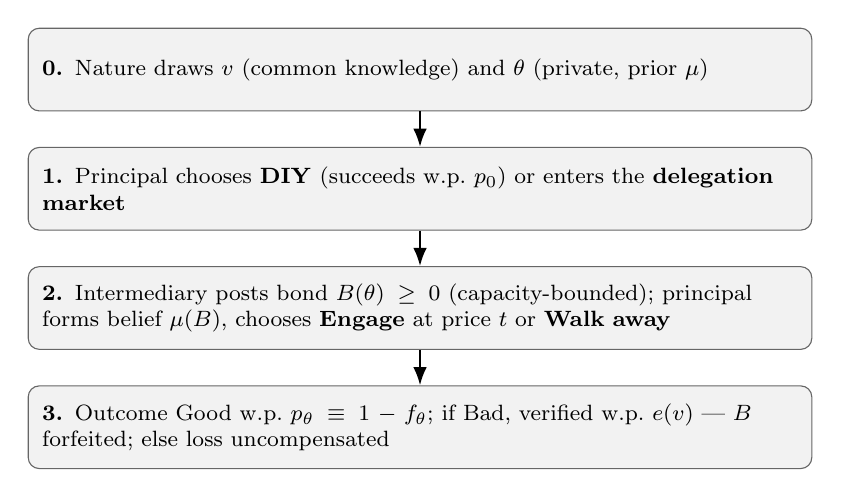
\begin{tikzpicture}[
  node distance=0.45cm,
  every node/.style={font=\footnotesize},
  stepbox/.style={rectangle, rounded corners, draw=black!60, fill=black!5,
    text width=9.6cm, minimum height=1.05cm, align=left, inner sep=5pt}
]
\node[stepbox] (n0) {\textbf{0.} Nature draws $v$ (common knowledge) and $\theta$ (private, prior $\mu$)};
\node[stepbox, below=of n0] (n1) {\textbf{1.} Principal chooses \textbf{DIY} (succeeds w.p.\ $p_0$) or enters the \textbf{delegation market}};
\node[stepbox, below=of n1] (n2) {\textbf{2.} Intermediary posts bond $B(\theta)\ge0$ (capacity-bounded); principal forms belief $\mu(B)$, chooses \textbf{Engage} at price $t$ or \textbf{Walk away}};
\node[stepbox, below=of n2] (n3) {\textbf{3.} Outcome Good w.p.\ $p_\theta\equiv1-f_\theta$; if Bad, verified w.p.\ $e(v)$ --- $B$ forfeited; else loss uncompensated};
\draw[-{Latex}, thick] (n0) -- (n1);
\draw[-{Latex}, thick] (n1) -- (n2);
\draw[-{Latex}, thick] (n2) -- (n3);
\end{tikzpicture}
\end{center}
\end{frame}

%----------------------------------------------------------------------
\begin{frame}{Two ways to get the task done: outcomes and payoffs}
\begin{center}
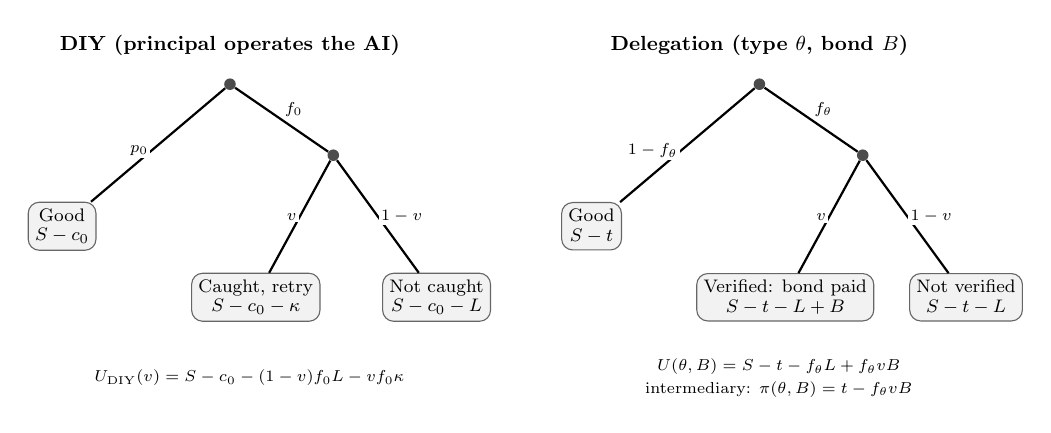
\begin{tikzpicture}[scale=0.82, transform shape,
  every node/.style={font=\footnotesize},
  ch/.style={circle, fill=black!70, inner sep=1.8pt},
  leaf/.style={rectangle, rounded corners, draw=black!60, fill=black!5, inner sep=3pt, align=center},
  lab/.style={font=\scriptsize, fill=white, inner sep=1pt},
  edge/.style={thick}
]
% ---- DIY (left) ----
\node[font=\small\bfseries] at (0,0.6) {DIY (principal operates the AI)};
\node[ch] (a0) at (0,0) {};
\node[leaf] (aG) at (-2.6,-2.2) {Good\\[-1pt]$S-c_0$};
\node[ch] (aB) at (1.6,-1.1) {};
\node[leaf] (aC) at (0.4,-3.3) {Caught, retry\\[-1pt]$S-c_0-\kappa$};
\node[leaf] (aN) at (3.2,-3.3) {Not caught\\[-1pt]$S-c_0-L$};
\draw[edge] (a0) -- node[lab,pos=0.55,left] {$p_0$} (aG);
\draw[edge] (a0) -- node[lab,pos=0.5,above right] {$f_0$} (aB);
\draw[edge] (aB) -- node[lab,pos=0.5,left] {$v$} (aC);
\draw[edge] (aB) -- node[lab,pos=0.5,right] {$1-v$} (aN);
\node[align=center,font=\scriptsize] at (0.3,-4.55) {$\UDIY(v)=S-c_0-(1-v)f_0L-vf_0\kappa$};

% ---- Delegation (right) ----
\begin{scope}[visible on=<2->]
\node[font=\small\bfseries] at (8.2,0.6) {Delegation (type $\theta$, bond $B$)};
\node[ch] (b0) at (8.2,0) {};
\node[leaf] (bG) at (5.6,-2.2) {Good\\[-1pt]$S-t$};
\node[ch] (bB) at (9.8,-1.1) {};
\node[leaf] (bV) at (8.6,-3.3) {Verified: bond paid\\[-1pt]$S-t-L+B$};
\node[leaf] (bN) at (11.4,-3.3) {Not verified\\[-1pt]$S-t-L$};
\draw[edge] (b0) -- node[lab,pos=0.55,left] {$1-f_\theta$} (bG);
\draw[edge] (b0) -- node[lab,pos=0.5,above right] {$f_\theta$} (bB);
\draw[edge] (bB) -- node[lab,pos=0.5,left] {$v$} (bV);
\draw[edge] (bB) -- node[lab,pos=0.5,right] {$1-v$} (bN);
\node[align=center,font=\scriptsize] at (8.5,-4.55) {$U(\theta,B)=S-t-f_\theta L+f_\theta vB$\\[2pt]intermediary: $\pi(\theta,B)=t-f_\theta vB$};
\end{scope}
\end{tikzpicture}
\end{center}
\end{frame}

%----------------------------------------------------------------------
\begin{frame}{Payoffs: DIY}
\begin{itemize}
  \item $f_0\equiv1-p_0$ --- principal's own (non-expert) failure probability.
  \item $c_0$ --- his cost of operating the AI directly.
  \item $\kappa$ --- cost of a successful retry when inspection catches a Bad draw (Assumption~3, next slides).
\end{itemize}
\vfill
\begin{equation*}
  \UDIY(v) = S-(1-v)f_0L-c_0-vf_0\kappa
\end{equation*}
\vfill
\begin{itemize}
  \item Affine in $v$: $\UDIY(v)=S-f_0L-c_0+v\,f_0(L-\kappa)$.
  \item In the leading case $L>\kappa$ (stake exceeds retry cost), $\UDIY$ is \alert{increasing} in $v$: better verification makes catch-and-retry more valuable.
\end{itemize}
\end{frame}

%----------------------------------------------------------------------
\begin{frame}{Payoffs: delegation}
Principal engages an intermediary of type $\theta$ who has posted bond $B$:
\begin{align*}
  \pi(\theta,B) &= t - f_\theta\, e(v)\, B \qquad\text{(intermediary)} \\[4pt]
  U(\theta,B) &= S-t-f_\theta L + f_\theta\, e(v)\, B \qquad\text{(principal)}
\end{align*}
\vfill
\begin{itemize}
  \item $\Ubar$ --- principal's outside option. Held fixed in \S3 (baseline); from \S3.3 on, $\Ubar=\UDIY(v)$.
  \item Types are ordered: $\fL>\fH>0$.
\end{itemize}
\end{frame}

%----------------------------------------------------------------------
\begin{frame}{Notation, at a glance}
\small
\begin{table}
\begin{tabular}{ll}
\toprule
$\theta\in\{\Ht,\Lt\}$, $\mu=\Pr(\Ht)$ & type, prior \\
$p_\theta$, $f_\theta\equiv1-p_\theta$ & success / failure probability by type, $\fL>\fH$ \\
$t$ & price paid to the intermediary (exogenous, common) \\
$B$ & bond posted by the intermediary \\
$e(v)$ & $\Pr(\text{verified}\mid\text{Bad})$ --- enforcement, $=v$ in the baseline \\
$\wbar$ & capacity bound on the bond $\Ht$ can credibly post \\
$S$, $L$ & task value if Good; stake destroyed if Bad \\
$v$ & principal's own verification precision \\
$p_0$, $f_0\equiv1-p_0$ & DIY success / failure probability \\
$c_0$, $\kappa$ & DIY operating cost; cost of a caught-and-redone retry \\
$\Ubar$ & principal's outside option \\
\bottomrule
\end{tabular}
\end{table}
\end{frame}

%----------------------------------------------------------------------
\begin{frame}{Assumptions 1--2}
\begin{exampleblock}{Assumption 1 (Fixed price)}
The price $t$ is exogenous and common to both intermediary types.
\end{exampleblock}
Type affects the probability of success, not the price of operating the AI --- consistent with raw AI execution itself being commoditized.
\vfill
\begin{exampleblock}{Assumption 2 (Common knowledge of verifiability)}
$v$ is known to both parties before the bond is posted.
\end{exampleblock}
Without it, the principal's DIY outside option, which depends on $v$, would be \emph{his} private information: the intermediary would be uncertain about the principal's participation threshold as well. Private information on both sides, instead of one.
\end{frame}

%----------------------------------------------------------------------
\begin{frame}{Assumption 3}
\begin{exampleblock}{Assumption 3 (Mode-specific remedy)}
A caught Bad draw is remedied differently depending on who operates the AI. Under DIY, the principal redoes the work himself at cost $\kappa$. Under delegation, the principal cannot redo the intermediary's work; his remedy is the bond.
\end{exampleblock}
\vfill
\begin{itemize}
  \item Retry is the principal's self-correction technology; the bond is delegation's remedy.
  \item Reflects what each party brings: the principal can redo \emph{his own} work when he catches a failure; what an intermediary offers is a higher probability of getting it right the \emph{first} time.
  \item This is the substantive reason the model builds two separate mechanisms (retry, bond) rather than one.
\end{itemize}
\end{frame}

%----------------------------------------------------------------------
\begin{frame}{Assumption 4}
\begin{exampleblock}{Assumption 4 (Capacity bound)}
The genuine type cannot credibly post a bond larger than $\wbar$.
\end{exampleblock}
\vfill
\begin{itemize}
  \item The judgment-proof problem, applied to the credibility of the \emph{signal itself}, not merely to ex post compensation.
\end{itemize}
\end{frame}

%----------------------------------------------------------------------
\begin{frame}{Assumption 5, and the enforcement technology}
\begin{exampleblock}{Assumption 5 (Equilibrium selection)}
We focus on (i) pooling without a bond, if it clears the principal's participation constraint; otherwise (ii) the least-cost separating equilibrium, if it exists. Where neither exists, separation fails, and we do not characterize the outcome.
\end{exampleblock}
\begin{itemize}
  \item Both rules are \emph{selections}. Pooling at a positive bond can coexist with separation for some priors; we set it aside, since it asks the genuine type to pay for a bond that does not distinguish it from the wrapper.
\end{itemize}
\vfill
\begin{block}{Enforcement technology}
$e(v)=v$ --- the most direct reading of ``if it's hard for the principal to verify, it's hard for a court to verify too'' as \emph{one} primitive. A general affine form, $e(v)=e_0+(1-e_0)v$, changes only the capacity threshold of \S4.
\end{block}
\end{frame}

%======================================================================
\section{Baseline Results}
%======================================================================

\begin{frame}{3.1 --- Set-up}
Suppose momentarily the intermediary is a \alert{single, known} type, succeeding with probability $p_1$ (compare the principal's own $p_0$).
\vfill
\begin{itemize}
  \item For a given verification level $v$: does the principal prefer to delegate at the posted price, or do it himself?
  \item Not yet about liability at all --- there is nothing to signal when type is known.
\end{itemize}
\end{frame}

%----------------------------------------------------------------------
\begin{frame}{Proposition 1 (make-or-buy)}
\begin{exampleblock}{\PropTitle{1}}
Suppose $p_1$ is known and $L>\kappa$. There is a unique threshold
\begin{equation*}
  v^{*} = \frac{\Delta p\cdot L-\Delta c}{f_0\,(L-\kappa)},\qquad \Delta p\equiv p_1-p_0,\quad \Delta c\equiv t-c_0,
\end{equation*}
below which delegating strictly beats DIY, above which delegation cannot beat DIY.
\end{exampleblock}
\end{frame}

%----------------------------------------------------------------------
\begin{frame}{Proposition 1 --- derivation}
No type uncertainty $\Rightarrow$ nothing to signal $\Rightarrow$ under Assumption 1, a bond is a pure transfer the intermediary dislikes, so $B=0$:
\begin{equation*}
  \UDEL = S-t-f_1L, \qquad f_1\equiv1-p_1 \quad\text{(flat in $v$, no retry term by Assumption 3)}
\end{equation*}
\pause
DIY is affine and, in the leading case, increasing in $v$:
\begin{equation*}
  \UDIY(v) = S-f_0L-c_0+v\,f_0(L-\kappa)
\end{equation*}
\pause
Their difference is affine with slope $-f_0(L-\kappa)<0$ when $L>\kappa$:
\begin{equation*}
  \UDEL-\UDIY(v) = \Delta p\cdot L-\Delta c-v\,f_0(L-\kappa)
\end{equation*}
\pause
Exactly one sign change $\Rightarrow$ the threshold $v^*$ above. $\square$
\end{frame}

%----------------------------------------------------------------------
\begin{frame}{Proposition 1 --- intuition}
\begin{columns}
\begin{column}{0.55\textwidth}
\begin{itemize}
  \item High verifiability makes catch-and-retry a \alert{substitute} for expertise: if a bad draw is cheaply caught and redone, you don't need someone who gets it right the first time.
  \item Low verifiability makes retry worthless --- you can't tell Good from Bad --- collapsing the comparison to a static ``is the quality premium worth the price premium'' calculation.
  \item That static comparison is exactly the terrain on which a credence-good unraveling problem can bite.
\end{itemize}
\end{column}
\begin{column}{0.45\textwidth}
\centering
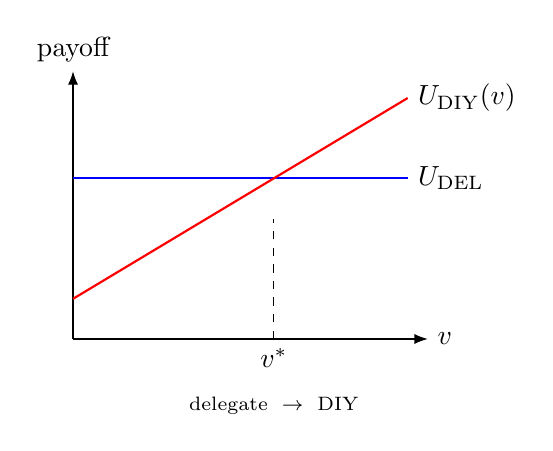
\begin{tikzpicture}[scale=0.85]
\draw[-{Latex}] (0,0) -- (5.3,0) node[right]{$v$};
\draw[-{Latex}] (0,0) -- (0,4) node[above]{payoff};
\draw[thick, blue] (0,2.4) -- (5,2.4) node[right,black]{$\UDEL$};
\draw[thick, red] (0,0.6) -- (5,3.6) node[right,black]{$\UDIY(v)$};
\draw[dashed] (3.0,0) -- (3.0,1.8);
\node[below] at (3.0,0) {$v^{*}$};
\node[align=center, below=4pt] at (3.0,-0.55) {\scriptsize delegate $\;\to\;$ DIY};
\end{tikzpicture}
\end{column}
\end{columns}
\end{frame}

%----------------------------------------------------------------------
\begin{frame}{3.2 --- The bond as a signal}
Now: type uncertainty, fixed enforcement $e$, fixed outside option $\Ubar$.
\vfill
\begin{itemize}
  \item Marginal cost of posting bond $B$ to type $\theta$: $\partial(f_\theta e B)/\partial B = f_\theta e$ --- \alert{strictly lower for $\Ht$}, since $\fL>\fH$.
  \item That gap alone --- not an assumed cost-of-effort asymmetry --- is single crossing, and it's derived from one primitive: each type's own probability of a bad draw.
\end{itemize}
\end{frame}

%----------------------------------------------------------------------
\begin{frame}{Proposition 2 (the bond)}
\begin{exampleblock}{\PropTitle{2}}
Suppose a known wrapper is not worth engaging even at a zero fee, $S-\fL L\le\Ubar$. The least-cost bond separating $\Ht$ from $\Lt$ is
\begin{equation*}
  \BH = \frac{t}{\fL\, e},
\end{equation*}
and $\Ht$ is always willing to post it.
\end{exampleblock}
\vfill
\begin{itemize}
  \item The condition $S-\fL L\le\Ubar$ is the \emph{scope} of the result, not an assumption of the model: it says a wrapper that reveals itself is not worth engaging, so it earns zero. In the nested model it reads $v\ge\vW$ (\S3.3).
\end{itemize}
\end{frame}

%----------------------------------------------------------------------
\begin{frame}{Proposition 2 --- derivation}
\small
A revealed wrapper is engaged at bond $B$ iff $S-t-\fL L+\fL eB\ge\Ubar$. At the smallest such bond it earns
\begin{equation*}
  t-\fL eB = S-\fL L-\Ubar \;\le\; 0
\end{equation*}
so an identified $\Lt$'s payoff is \alert{0}. (This is where the scope condition is used.)
\pause
\vspace{4pt}
Mimicking $\Ht$'s bond is therefore deterred exactly when
\begin{equation*}
  t-\fL eB\le 0 \;\iff\; B\ge\frac{t}{\fL e}
\end{equation*}
\pause
$\Ht$ wants the \emph{smallest} such bond (bonding is costly): $\BH=t/(\fL e)$. Higher separating bonds exist too, but the standard refinement (Riley; Cho and Kreps) selects the least-cost one.
\pause
\vspace{4pt}
Check $\Ht$'s own participation:
\begin{equation*}
  t-\fH e\BH = t\Big(1-\frac{\fH}{\fL}\Big) > 0 \qquad\text{automatic, given } \fL>\fH. \quad\square
\end{equation*}
\end{frame}

%----------------------------------------------------------------------
\begin{frame}{Proposition 3 (invariance to enforcement)}
\small
\begin{exampleblock}{\PropTitle{3}}
At $\BH$, the principal's payoff does not depend on $e$:
\begin{equation*}
  \frac{\partial U(\Ht,\BH)}{\partial e}=0,
\end{equation*}
provided enforcement is costless to run.
\end{exampleblock}
\vfill
\textbf{Derivation --- one substitution:}
\begin{equation*}
  U(\Ht,\BH) = S-t-\fH L + \fH e\cdot\frac{t}{\fL e} = S-t-\fH L+\frac{\fH t}{\fL}
\end{equation*}
$e$ \alert{cancels exactly} between the grossed-up bond and the recovery term. $\square$
\vfill
\begin{itemize}
  \item \textbf{Intuition:} worse enforcement inflates the nominal bond exactly enough to offset the lower chance of collecting it, so better courts make separation more \emph{feasible}, not more valuable; feasibility is where the capacity bound of \S4 enters.
\end{itemize}
\end{frame}

%----------------------------------------------------------------------
\begin{frame}{Proposition 4 (pooling threshold)}
\begin{exampleblock}{\PropTitle{4}}
Pooling at $B=0$ clears the principal's participation constraint iff $\mu\ge\mu^{*}$, where
\begin{equation*}
  \mu^{*} = \frac{\fL-\dfrac{S-t-\Ubar}{L}}{\fL-\fH}.
\end{equation*}
\end{exampleblock}
\vfill
\textbf{Derivation.} At $B=0$, posterior $=$ prior, so
\begin{equation*}
  U_{\mathrm{pool}}(\mu) = S-t-[\mu\fH+(1-\mu)\fL]L, \qquad \text{increasing in } \mu \text{ since } \fH<\fL.
\end{equation*}
Set $U_{\mathrm{pool}}(\mu)=\Ubar$, solve for $\mu$. $\square$
\vfill
\begin{itemize}
  \item If the prior is good enough, the principal is willing to engage even without separation.
\end{itemize}
\end{frame}

%----------------------------------------------------------------------
\begin{frame}{Proposition 4 --- intuition}
\begin{itemize}
  \item Above $\mu^*$, $\Ht$ has no reason to signal: already engaged at $B=0$ earning $t$; any bond only lowers that.
  \item Follows from \textbf{Assumption 1} (fixed price): unlike Spence (1973), being identified as $\Ht$ is worth \emph{nothing} beyond being engaged, because the price doesn't respond to belief.
\end{itemize}
\end{frame}

%----------------------------------------------------------------------
\begin{frame}{3.3 --- Nesting the two}
\small
Substitute $\Ubar=\UDIY(v)$ and $e(v)=v$ into Propositions 2--4: the delegation market, screened by a bond, evaluated against an outside option that depends on the \emph{same} verification parameter.
\vfill
Define the principal's expected shortfall at $v=0$, relative to a wrapper working for free:
\begin{equation*}
  \Delta \equiv Lf_0+c_0-L\fL
\end{equation*}
Proposition 2's scope condition, $S-\fL L\le\UDIY(v)$, becomes $v\ge\vW\equiv\Delta/[f_0(L-\kappa)]$.
\vfill
\begin{itemize}
  \item \textbf{Why $\vW$:} $S-\fL L$ is what a wrapper working for free would deliver. $\UDIY(v)$ rises with $v$, so it overtakes that at $\vW$. Below $\vW$, even a known wrapper is worth hiring for the principal, if it posts a large enough bond. So a wrapper that reveals itself still earns a positive payoff, and the logic of Prop.\ 2 (mimicking is deterred because a revealed wrapper earns nothing) fails.
\end{itemize}
\end{frame}

%----------------------------------------------------------------------
\begin{frame}{Proposition 5 (the separating band)}
\begin{exampleblock}{\PropTitle{5}}
Suppose $L>\kappa$. Then
\begin{equation*}
  \mu^{*}(v)=\frac{\fL-f_0+\frac{t-c_0}{L}+v\,\frac{f_0(L-\kappa)}{L}}{\fL-\fH},\qquad
  \vIR=\frac{f_0L+c_0-t-\fH L+\fH t/\fL}{f_0(L-\kappa)}
\end{equation*}
with $\mu^*(v)$ affine and increasing in $v$. Four regions:
\begin{enumerate}
  \item[(a)] \emph{Pooling without a bond:} $\mu\ge\mu^*(v)$.
  \item[(b)] \alert{Separating band:} $\mu<\mu^*(v)$, $\vW\le v\le\vIR$. $\Ht$ separates at $\BH$.
  \item[(c)] \emph{No separation:} $\mu<\mu^*(v)$, $v<\vW$.
  \item[(d)] \emph{DIY:} $v>\vIR$. Delegation cannot beat DIY.
\end{enumerate}
\end{exampleblock}
\end{frame}

%----------------------------------------------------------------------
\begin{frame}{Proposition 5 --- derivation highlights}
Substituting $\Ubar=\UDIY(v)$ into Proposition 4's $\mu^*$ gives an affine map (algebra: direct substitution, slope $f_0(L-\kappa)/[L(\fL-\fH)]>0$).
\pause
\vspace{6pt}
By Proposition 3, $U(\Ht,\BH)$ is \alert{flat} in $v$; $\UDIY(v)$ is increasing. They cross once, at $\vIR$.
\pause
\vspace{6pt}
Below $\vW$, an identified wrapper can obtain engagement and earn $S-\fL L-\UDIY(v)>0$: the deterrence argument of Proposition 2 fails, so there is no separation.
\end{frame}

%----------------------------------------------------------------------
\begin{frame}{Proposition 5 --- intuition}
\begin{columns}[T]
\begin{column}{0.54\textwidth}
\small
\begin{itemize}
  \item \textbf{Pooling without a bond} ($\mu\ge\mu^*(v)$): the prior is good enough for the principal to engage with no bond. $\mu^*(v)$ rises with $v$, because the DIY outside option improves.
  \item \alert{Separating band}: $\Ht$ separates at $\BH$. Upper edge $\vIR$: Prop.\ 1 plus the bond.
  \item \textbf{No separation} ($v<\vW$): imitation is too good to screen out, even if $\Ht$ can post any bond.
  \item \textbf{DIY} ($v>\vIR$): catch-and-retry makes identifying an expert unnecessary.
\end{itemize}
\end{column}
\begin{column}{0.46\textwidth}
\centering
\includegraphics[width=\textwidth]{figures/regions_baseline.pdf}

\scriptsize Example of the last slides, $t=1.2$
\end{column}
\end{columns}
\end{frame}

%======================================================================
% No section page for section 4 (removed at Ricardo's request)
\metroset{sectionpage=none}
\section{Capital-Constrained Bonding}
\metroset{sectionpage=progressbar}
%======================================================================

\begin{frame}{Reintroducing Assumption 4}
\begin{itemize}
  \item We now impose the capacity bound: $\Ht$ cannot post a bond larger than $\wbar$.
  \item The question: how does a limit on the bond change the separating band of Proposition 5?
\end{itemize}
\end{frame}

%----------------------------------------------------------------------
\begin{frame}{Proposition 6 (band with capital constraint)}
\begin{exampleblock}{\PropTitle{6}}
Separation at $\BH$ is feasible only if $\BH\le\wbar$, i.e.\ $v\ge\vcap\equiv t/(\fL\wbar)$. Under $e(v)=v$, the separating band becomes
\begin{equation*}
  \mu<\mu^*(v),\qquad \max\{\vW,\vcap\}\le v\le\vIR,
\end{equation*}
and is empty if $\vcap>\vIR$. For $\mu<\mu^*(v)$ and $v<\max\{\vW,\vcap\}$ there is no separation. The pooling and DIY regions of Proposition 5 are unchanged.
\end{exampleblock}
\end{frame}

%----------------------------------------------------------------------
\begin{frame}{Proposition 6 --- derivation}
\begin{equation*}
  \BH=\frac{t}{\fL v}\le\wbar \;\iff\; v\ge\vcap=\frac{t}{\fL\wbar} \qquad\text{--- a vertical line in $(v,\mu)$ space.}
\end{equation*}
\pause
Combined with Proposition 5, $\Ht$ separates iff $\mu<\mu^*(v)$ and $\max\{\vW,\vcap\}\le v\le\vIR$.
\end{frame}

%----------------------------------------------------------------------
\begin{frame}{Proposition 6 --- intuition}
\begin{itemize}
  \item The less verifiable the task, the larger the bond needed to deter the wrapper ($\BH=t/(\fL v)$).
  \item The bond cannot exceed the expert's capital, so verifiability must be \alert{high enough} for the bond to be payable.
  \item And it must be \alert{low enough} that the principal does not simply do the task himself.
  \item Between the two, separation is possible: that is the band.
\end{itemize}
\end{frame}

%----------------------------------------------------------------------
\begin{frame}{The $(v,\mu)$ map}
\begin{figure}
\centering
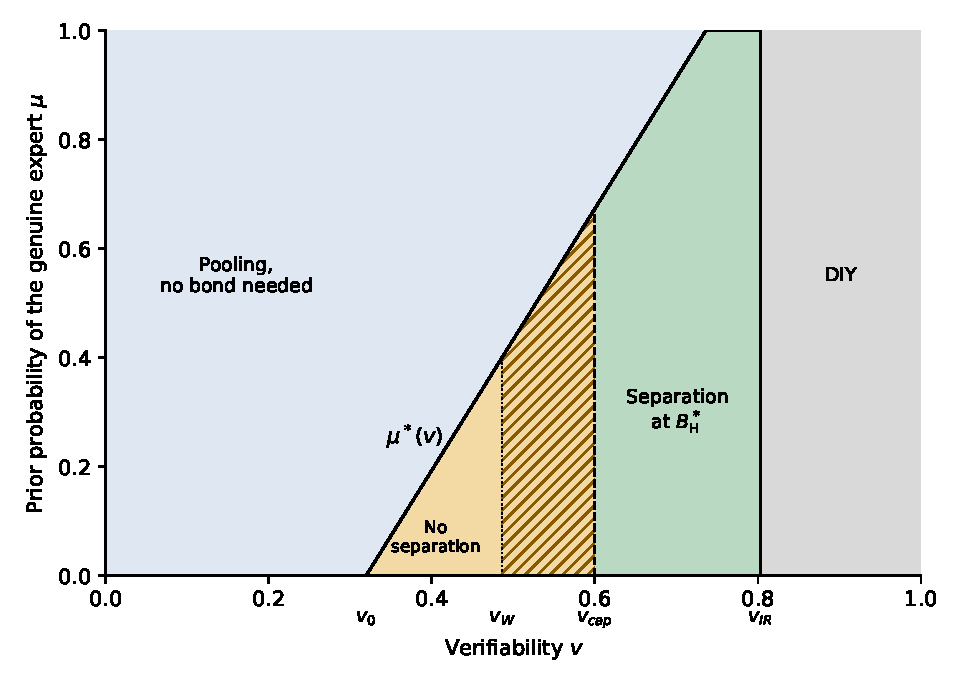
\includegraphics[width=0.46\textwidth]{figures/regions.pdf}
\end{figure}
\vspace{-4pt}
\begin{center}
\scriptsize Example: $\fH=0.2,\ \fL=0.5,\ f_0=0.8,\ L=10,\ \kappa=1,\ c_0=0.5,\ \wbar=4,\ S=20,\ t=1.2$, giving $\vW=0.486$, $\vcap=0.600$, $\vIR=0.803$. The hatched strip $[\vW,\vcap)$ is where separation would occur if the expert could post any bond, and is lost to the capital constraint.
\end{center}
\end{frame}

%----------------------------------------------------------------------

%======================================================================
\section{Discussion, Extensions, and Conclusion}
%======================================================================


%----------------------------------------------------------------------
\begin{frame}{Implications, a conjecture, and a caveat}
\small
\begin{itemize}
  \item \textbf{Implications.} Better imitation (lower $\fL$) raises $\vW$ and $\vcap$. More bonding capacity lowers $\vcap$.
  \vspace{6pt}
  \item \textbf{Conjecture (not derived).} Where separation fails, the market cannot tell experts from imitators, and with a fixed price it does not reward expertise: it will eventually lose it.
  \vspace{6pt}
  \item \textbf{Caveat.} Assumption 5 selects separation wherever pooling without a bond is not enough. Pooling clears the principal's IR only in expectation; a principal who cannot be compensated by a transfer, or is judged ex post, may reject it.
\end{itemize}
\end{frame}

%----------------------------------------------------------------------
\begin{frame}{Extensions}
\begin{itemize}
  \item \textbf{Costly bonds.} Real bonds carry costs $\propto$ face value (surety premiums, LC fees, collateral opportunity cost). Since $\BH\propto1/e$, weaker enforcement makes separation more wasteful even when affordable --- Prop.\ 3's invariance breaks.
  \vspace{6pt}
  \item \textbf{Liability as one signal among several.} Reputation, credentials, institutional affiliation are alternatives with their own verification requirements, and AI erodes them through different channels; not compared here.
  \vspace{6pt}
  \item \textbf{Risk and the ex-post cost of pooling.} The expected-value IR constraint suits the intermediary's repeated-trial view but is strong for a one-shot principal, especially where harm is not restorable by a transfer. Replacing it with a risk-averse or ex-post welfare criterion is left for future work.
\end{itemize}
\end{frame}

%----------------------------------------------------------------------
\begin{frame}{Conclusion}
\footnotesize
Two mechanisms jointly determine whether a market for genuine expertise survives cheap, competent AI execution: \textbf{(i)} the principal's ability to catch and redo a bad result himself; \textbf{(ii)} a bond that lets genuine expertise be credibly signaled when he cannot.
\vfill
\begin{block}{}
The bond separates genuine expertise from imitation only in an \textbf{intermediate band of verifiability}.
\end{block}
\vspace{2pt}
\begin{itemize}
  \item Above the band, the principal does the task himself. Below it, a wrapper cannot be screened out.
  \item A limit on the capital a genuine expert can post raises the band's lower edge further.
  \item Better imitation, which AI gives the wrapper, raises the edge; more bonding capacity lowers it wherever capital sets it.
  \item Where separation fails, the market cannot tell experts from imitators --- we conjecture it will not keep its experts.
\end{itemize}
\end{frame}

%----------------------------------------------------------------------
\begin{frame}{}
\vfill
\centering
\Large\textbf{Thank you --- questions and comments welcome.}
\vfill
\end{frame}

\end{document}
